% !TeX spellcheck = en_US
\section{Background and Domain Information}
\label{chapter:background}

The domain of our Semantic Data Warehouse is about inquiries from tourists that want to make holiday in South Tyrol. The main idea of this project, is to allow a drill-down into special attributes of the data warehouse (abbreviated ''DW'') connected to outside \textsc{SparQL} endpoints. 

\subsection{Business goals}

The given business goal of that DW is to provide metrics and statistics to support data driven decision making to improve tourist accommodation numbers in the future. However, it can be difficult for DW designers to find more details about dimensions in a data warehouse. Therefore, this project can help to investigate upon a dimension detail by adding a mapping from the DW table to any remote data source.

In summary, this project should provide three main functionalities:
\begin{itemize}
\item Querying an \textsc{Ontop} ontology through the \textsc{Quest OWL API}
\item Grouping these queries with the \texttt{GROUP BY} clause, and some aggregation functions
\item Joining the ontology with another outside ontology provided by an \textsc{SparQL} endpoint, i.e., \textit{dbpedia.org}
\end{itemize}

Unfortunately, during development I found out that, aggregation and the \texttt{SERVICE} keyword is currently not supported in \textsc{Ontop}, therefore the project goals are now as follows:
\begin{itemize}
\item Querying an \textsc{Ontop} ontology through the \textsc{Quest OWL API}
\item Aggregating the results with Java (currently only \textsc{Count} is supported) 
\item Querying another outside ontology provided by an \textsc{SparQL} endpoint, i.e., \textit{dbpedia.org}, when a destination town gets clicked in the result set of a previously executed query.
\end{itemize}

\subsection{Data set: Tourist inquiries}

\textit{Please note, that this data is \textbf{confidential}, and must not be used outside this project. The data set strings are partially German, and partially British, therefore ''Inquiry'' and ''Enquiry'' are meant to mean the same, i.e., concept or literal.}

The dataset provided by LTS has 837,648 entries, each one is a inquiry
a guest made. After data cleaning 837,463 tuples remain. The data covers the
inquiries made in the period between 2015-01-01 and 2016-09-05. The inquiries
regarding stay periods between 2015-01-02 and 2020-08-20.

The schema is the following:
\begin{itemize}
\item \textbf{arrival}, \textit{mandatory}, date the guest plans to arrive / check in
\item \textbf{departure}, \textit{mandatory}, date the guest plans to leave / check out
\item \textbf{country}, \textit{optional}, the home country of the guest, may be null
\item \textbf{adults}, \textit{optional}, the number of adults
\item \textbf{children}, \textit{optional}, the number of children
\item \textbf{destination}, \textit{mandatory}, the ISTAT municipality code of the interested lodging establishment\footnote{\url{https://en.wikipedia.org/wiki/Municipalities_of_South_Tyrol}}
\item \textbf{category}, \textit{mandatory}, the category of the lodging establishment 
\begin{enumerate}
\item Gastgewerbliche Betriebe: Hotel, Pensionen, Garni, Residence und Gasth\"ofe
(1-3 Sterne)
\item  Gastgewerbliche Betriebe: Hotel, Pensionen, Garni, Residence und Gasth\"ofe (4-5 Sterne) 
\item  Privatvermieter
\item  Bauernh\"ofe
\item Sonstiges
\end{enumerate} 
\item \textbf{submitted\_on}, \textit{mandatory}, the timestamp of the inquiry
\end{itemize}


\subsection{Schema: Tourist inquiries}
\label{chapter:schema}

In figure~\ref{fig:schema_fact_inquiry} is shown a first draft of the dimensional fact model of the fact enquiry.
The measures of the fact are the number of guests (adults and children), the
length of a stay duration. A simple version of the data warehouse fact schema is depicted in figure~\ref{fig:fact_schema}.

\begin{figure}
	\centering
	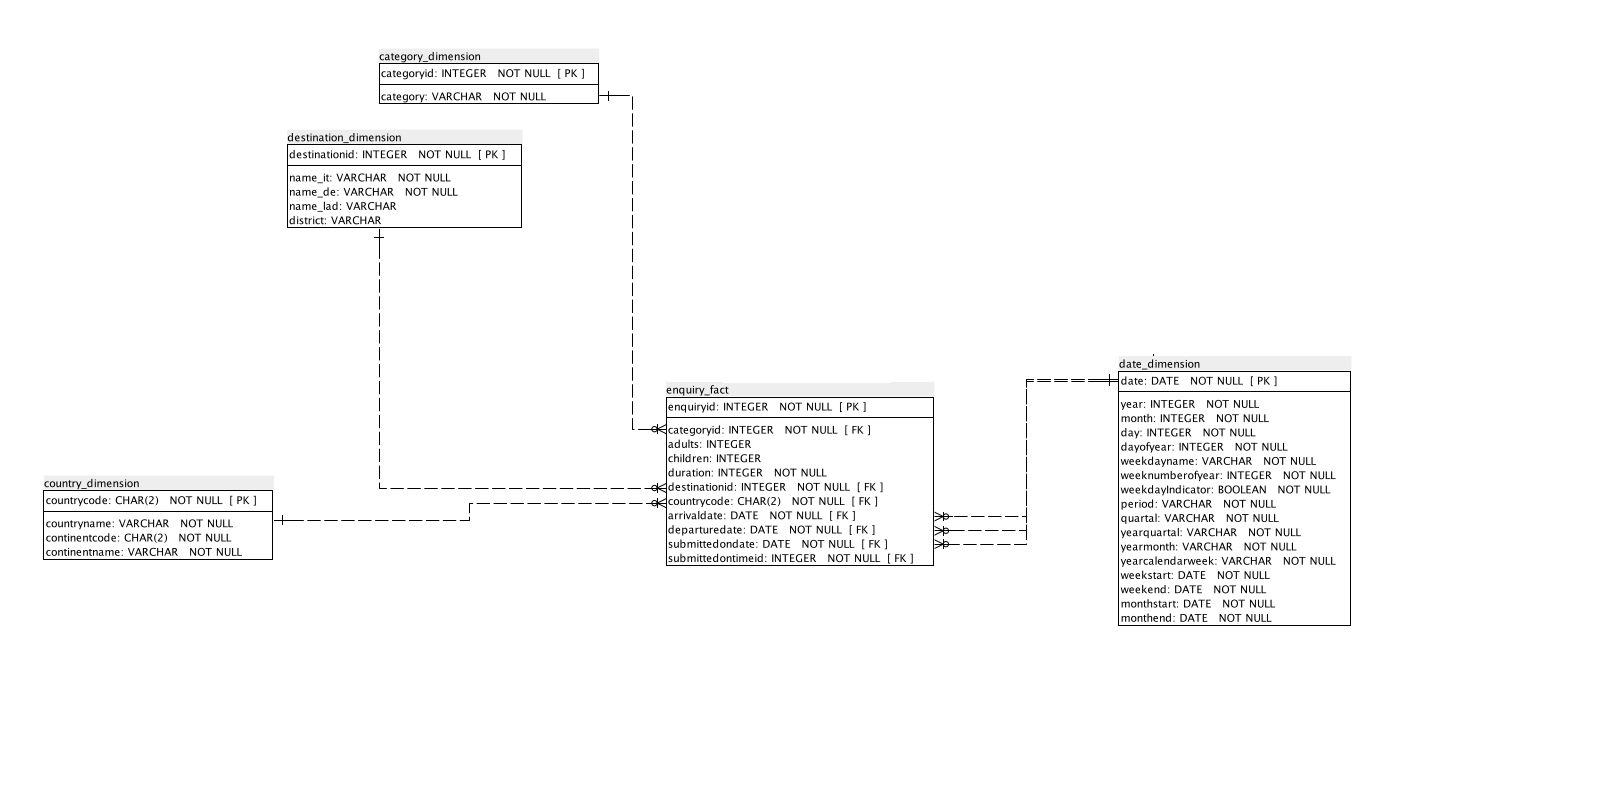
\includegraphics[scale=0.5,width=\textwidth]{img/schema_fact_inquiry.jpg}
	\caption{Relational schema of the fact INQUIRY (only dimensions and fact tables shown that have an \textsc{Ontop} mapping to the ontology)}
	\label{fig:schema_fact_inquiry}
\end{figure}

\begin{figure}
	\centering
	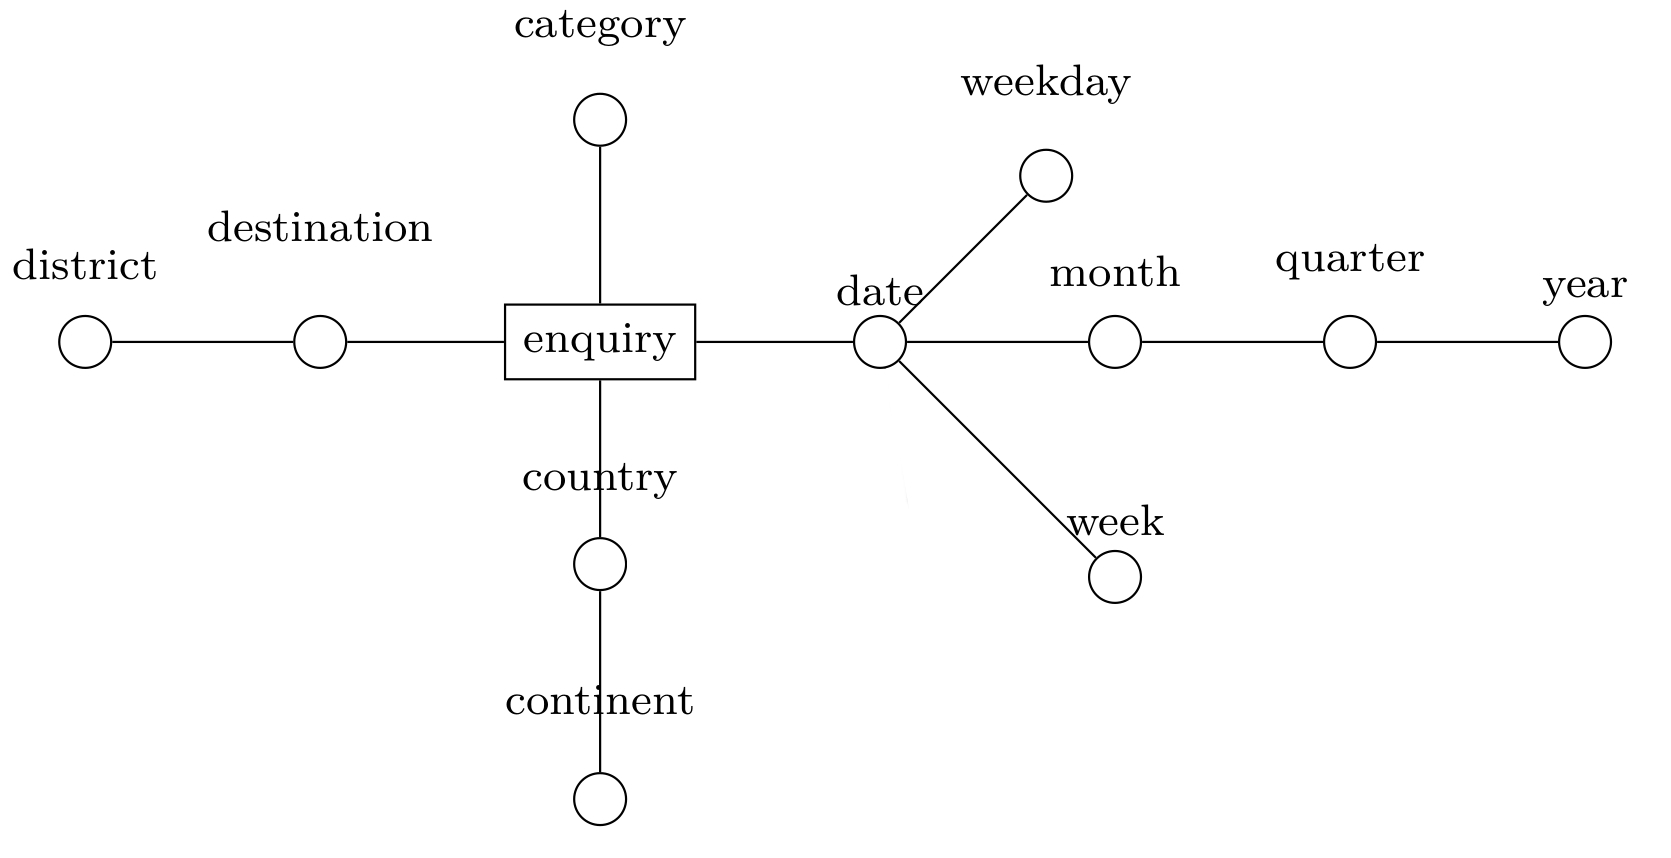
\includegraphics[scale=0.35,width=\textwidth]{img/fact_schema.jpg}
	\caption{Fact schema of the fact INQUIRY (only dimensions and fact tables shown that have an \textsc{Ontop} mapping to the ontology)}
	\label{fig:fact_schema}
\end{figure}
